%
% db-exponentialverteilung.tex -- Datenblatt der Exponentialverteilung
%
% (c) 2015 Prof Dr Andreas Mueller, Hochschule Rapperswil
%
\subsection{Steckbrief}
\begin{center}
\renewcommand{\arraystretch}{2}
\begin{tabular}{|l|l|}
\hline
Name&Exponentialverteilung\\
\hline
Dichtefunktion&$\displaystyle ae^{-ax}$,\quad $a>0$\\
Verteilungsfunktion&$1-e^{-ax}$\\
Erwartungswert&$\displaystyle \frac1a$\\
Varianz&$\displaystyle \frac1{a^2}$\\
Median&$\displaystyle \frac1a\log 2$\\[8pt]
$P(|X-E(X)|>\varepsilon)$&
\begin{minipage}{3.7in}
$
\begin{cases}
e^{-a\varepsilon-1}&\qquad\text{für $\varepsilon > \frac1a$}\\
1-e^{a\varepsilon-1}+e^{-a\varepsilon-1}&\qquad\text{für $\varepsilon \le \frac1a$}
\end{cases}
$
\end{minipage}
\\[10pt]
\hline
Anwendungen&\begin{minipage}{3.7in}%
\strut
$\bullet$ Prozess ohne Erinnerungsvermögen\\
$\bullet$ Radioaktivität
\strut
\end{minipage}\\
\hline
\end{tabular}
\end{center}

\subsection{Verteilungsfunktion und Wahrscheinlichkeitsdichte}
Verteilungsfunktion (oben) und Dichtefunktion (unten) der
Exponentialverteilung:
\begin{center}
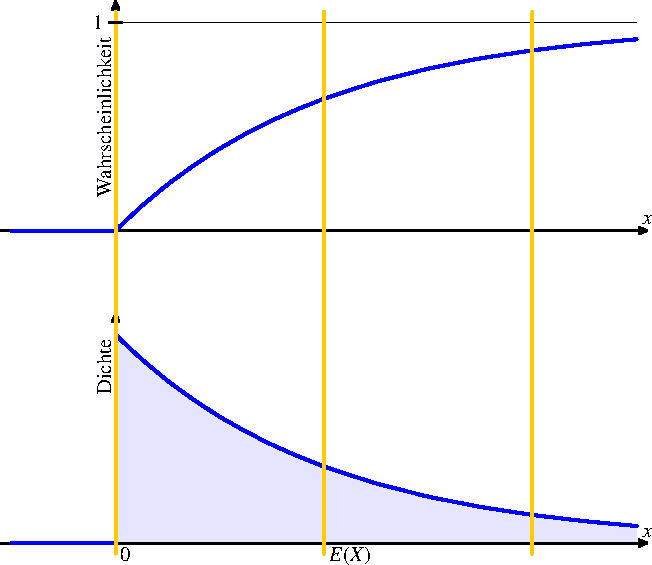
\includegraphics[width=0.8\hsize]{images/verteilungsfunktion-8}
\end{center}

\subsection{Wahrscheinlichkeit grosser Abweichungen}
Wahrscheinlichkeit für eine grosse Abweichung bei einer
Exponentialverteilten Zufallsvariable, oben die durch den Satz von Tschebyscheff
gegebene Schranke (grün), unten die exakte Rechnung mit
Hilfe der Exponentialvereteilung (rot):
\begin{center}
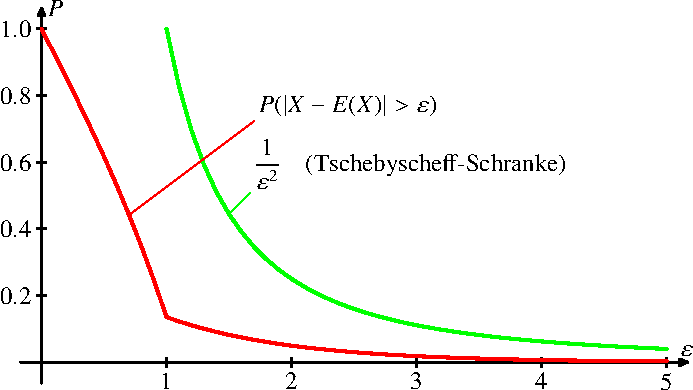
\includegraphics{images/exp-1.pdf}
\end{center}

\subsection{Parameter schätzen}
Der Parameter $1/a$ kann mit dem erwartungstreuen Schätzer
\[
\frac1{\hat a(x_1,\dots,x_n)}=\frac{x_1+\dots+x_n}n
\]
geschätzt werden.

\subsection{Erlang-Verteilungen}
Seien $X_i$ unabhängige, identisch mit Parameter $a$ exponentialverteilte
Zufallsvariablen.
Dann ist $X_1+\dots+X_n$ Erlang-verteilt. 
Die Erlang-Verteilungen wurden für die Analyse von Telefonzentralen erfunden,
und sind allgemein in der Queueing-Theorie nützlich.
Die Wahrscheinlichkeitsdichte und die Verteilungsfunktionen sind
\begin{align*}
F_{X_1+\dots+X_k}(x)&=\begin{cases}
\displaystyle 1-e^{-ax}\sum_{i=0}^{k-1}\frac{(ax)^i}{i!}&\qquad x\ge 0\\
\displaystyle 0&\qquad x < 0
\end{cases}
\\
\varphi_{X_1+\dots+X_k}(x)&=\begin{cases}
\displaystyle a^k\frac{x^{k-1}}{(k-1)!}e^{-ax}&\qquad x\ge 0\\
\displaystyle 0&\qquad x<0.
\end{cases}
\end{align*}
